\documentclass{beamer}

\usetheme{src/sintef}
\usefonttheme[onlymath]{serif}
\titlebackground*{beamerthemesrc/assets/background}
\setbeamertemplate{caption}[numbered]
%-------------add your packages here-------------
\usepackage[portuguese]{babel}
\usepackage{amsfonts,amsmath,oldgerm}
\usepackage{subfig}
\usepackage{graphicx}

\usepackage{tcolorbox}
\usepackage{adjustbox}
\usepackage{listings, listings-rust}

\usepackage{colortbl}
\usepackage{nicefrac, xfrac}

%-------------add your commands here-------------
\newcommand{\hrefcol}[2]{\textcolor{cyan}{\href{#1}{#2}}}
\newcommand{\testcolor}[1]{\colorbox{#1}{\textcolor{#1}{test}}~\texttt{#1}}

%-------------lst settings-----------------------

\colorlet{punct}{red!60!black}
\definecolor{background}{HTML}{EEEEEE}
\definecolor{delim}{RGB}{20,105,176}
\colorlet{numb}{magenta!60!black}
\definecolor{midgray}{gray}{.5}

\lstdefinelanguage{json}{
    basicstyle=\normalfont\ttfamily,
    stepnumber=1,
    numbersep=8pt,
    showstringspaces=false,
    breaklines=true,
    literate=
     *{0}{{{\color{numb}0}}}{1}
      {1}{{{\color{numb}1}}}{1}
      {2}{{{\color{numb}2}}}{1}
      {3}{{{\color{numb}3}}}{1}
      {4}{{{\color{numb}4}}}{1}
      {5}{{{\color{numb}5}}}{1}
      {6}{{{\color{numb}6}}}{1}
      {7}{{{\color{numb}7}}}{1}
      {8}{{{\color{numb}8}}}{1}
      {9}{{{\color{numb}9}}}{1}
      {:}{{{\color{punct}{:}}}}{1}
      {,}{{{\color{punct}{,}}}}{1}
      {\{}{{{\color{delim}{\{}}}}{1}
      {\}}{{{\color{delim}{\}}}}}{1}
      {[}{{{\color{delim}{[}}}}{1}
      {]}{{{\color{delim}{]}}}}{1},
}

\definecolor{template_brackes}{HTML}{0431FA}
\definecolor{template_keyword}{HTML}{859900}
\definecolor{template_magic_variable}{HTML}{268BD2}

\lstdefinelanguage{jinja2}{
    basicstyle=\normalfont\ttfamily,
    stepnumber=1,
    numbersep=8pt,
    showstringspaces=false,
    breaklines=true,
    literate=
     *{\{}{{{\color{template_brackes}\{}}}{1}
      {\}}{{{\color{template_brackes}\}}}}{1}
      {(}{{{\color{template_brackes}(}}}{1}
      {)}{{{\color{template_brackes})}}}{1}
      {\%}{{{\color{template_brackes}\%}}}{1}
      {loop}{{{\color{template_magic_variable}loop}}}{4}
      {recursive}{{{\color{template_keyword}recursive}}}{9}
      {if}{{{\color{template_keyword}if}}}{2}
      {else}{{{\color{template_keyword}else}}}{4}
      {for}{{{\color{template_keyword}for}}}{3}
      {endif}{{{\color{template_keyword}endif}}}{5}
      {endfor}{{{\color{template_keyword}endfor}}}{6}
      {set}{{{\color{template_keyword}set}}}{3}
      {not}{{{\color{template_keyword}not}}}{3}
      {[}{{{\color{delim}{[}}}}{1}
      {]}{{{\color{delim}{]}}}}{1},
}

%-------------title here--------------------
\title{Desenvolvimento de um software \textit{open source} para a modelagem e simulação do Sistema Imune Humano}
\subtitle{Exame de Qualificação}
\course{Mestrado em Ciência da Computação}
\author{
    \hrefcol{mailto:dev@brenno.codes}{Brenno Lemos}
    \and
    \hrefcol{mailto:alexandre.pigozzo@ufsj.edu.br}{Orientador:  Prof. Alexandre B. Pigozzo}
}
\IDnumber{}

%--------------begin document--------------------
\begin{document}
\maketitle

\section{Introdução}
\begin{frame}{Introdução}
\end{frame}


\section{Trabalhos Relacionados}
\begin{frame}{Trabalho Anterior — AC Designer}
    O trabalho que levou diretamente a este, AC-Designer, envolveu o desenvolvimento de um software para a criação e simulação de Autômatos Celulares. O software conta com várias funcionalidades que foram trazidas para este, como exportação de código e simulação \textit{onsite}.

    \begin{figure}
        \centering
    
        \subfloat{{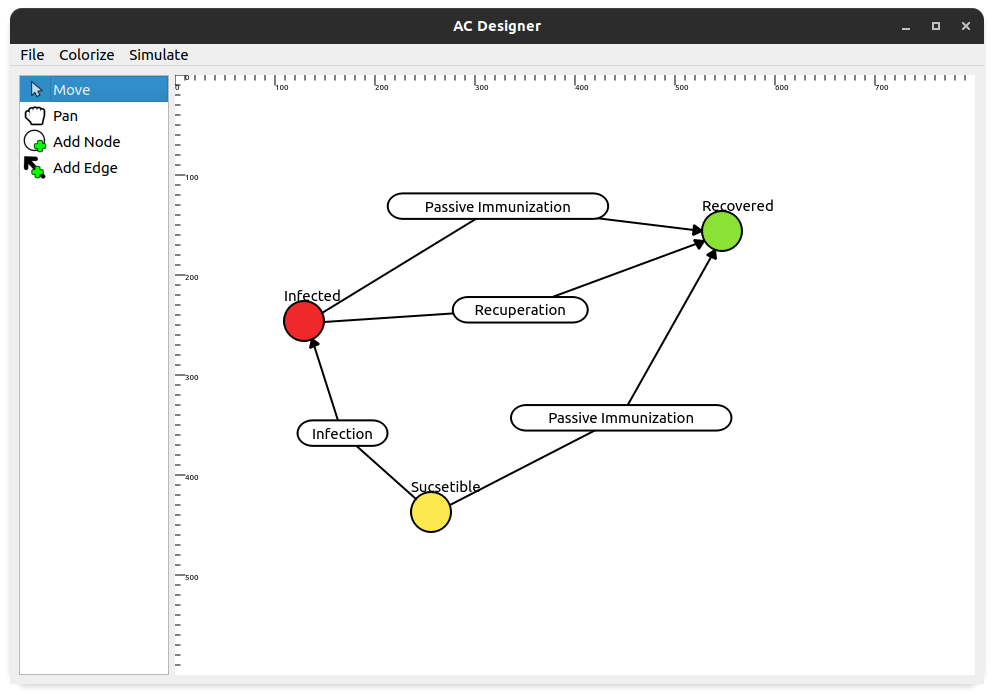
\includegraphics[width=.44\textwidth]{beamerthemesrc/images/ac-designer-sir.png}}}
        \quad
        \subfloat{{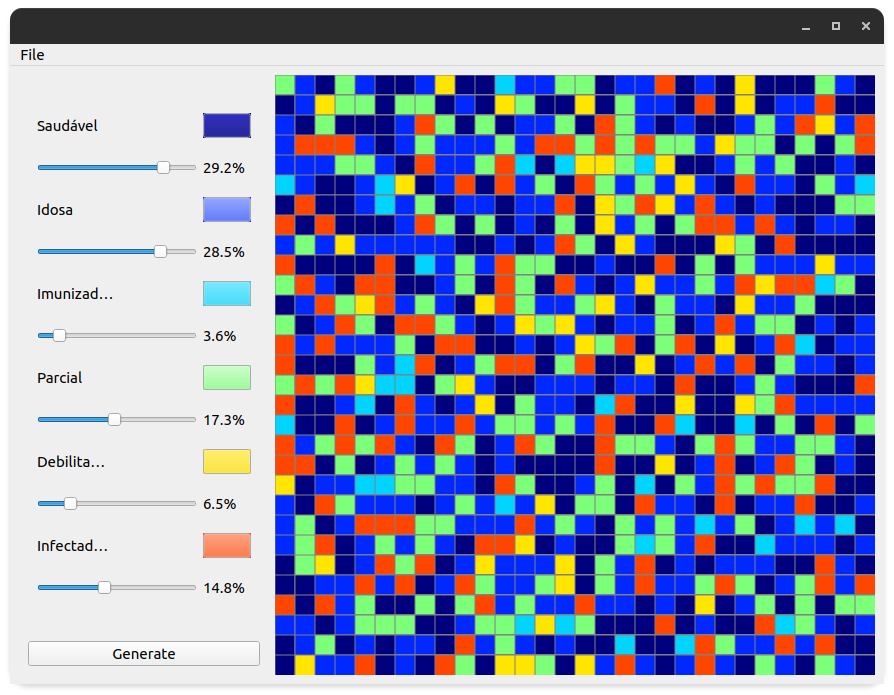
\includegraphics[width=.4\textwidth]{beamerthemesrc/images/ac-designer}}}
    
        \caption{Tela principal e de simulação do software.}
    \end{figure}
\end{frame}

\begin{frame}{Snoopy}
    \begin{itemize}
        \item Permite a modelagem de Redes de Petri;
        \item Utiliza uma representação baseada em grafos;
            \begin{itemize}
                \item Círculos representam estados (\textit{places}) e quadrados representam transições;
            \end{itemize}
        \item Foi uma grande inspiração às interfaces deste e do trabalho anterior, por ser simples de entender e representar;
        \item Assim como este trabalho, possui simulação \textit{onsite};
    \end{itemize}

    \begin{figure}
        \centering
    
        \subfloat{{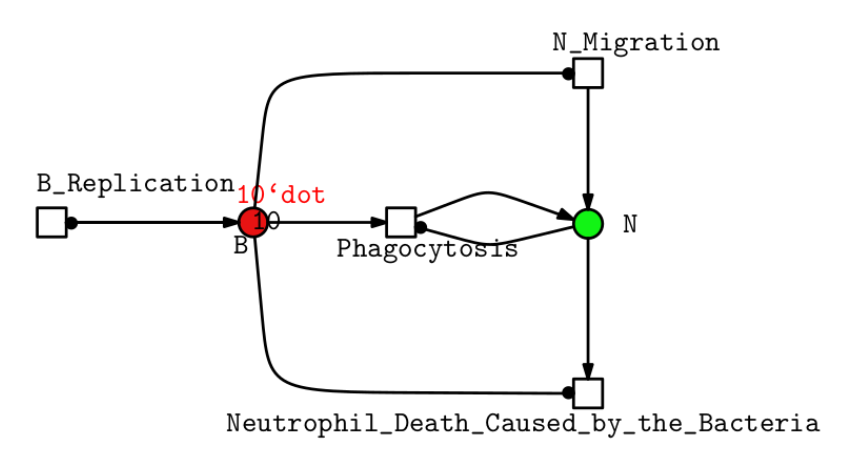
\includegraphics[width=.45\textwidth]{beamerthemesrc/images/snoopy-modelo.png}}}
        \quad
        \subfloat{{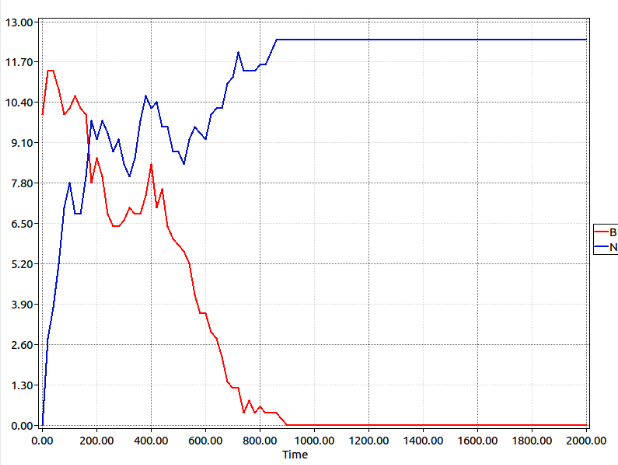
\includegraphics[width=.35\textwidth]{beamerthemesrc/images/snoopy-grafico.png}}}
    
        \caption{Exemplo de um modelo na interface e o resultado da simulação.}
    \end{figure}

\end{frame}

\begin{frame}{VCell e InsightMaker}

    \begin{columns}
        \begin{column}{.5\textwidth}
            \begin{itemize}
                \item O VCell é uma plataforma de modelagem de sistemas biológicos celulares;
                \item Os modelos são construídos com base em regras;
            \end{itemize}

            \begin{figure}
                \centering
                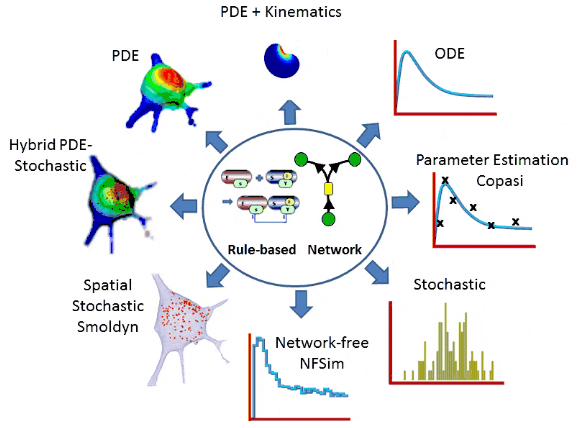
\includegraphics[width=.60\textwidth]{beamerthemesrc/images/vcell.png}
                \caption{Modelos suportados pelo VCell.}
            \end{figure}
        \end{column}

        \begin{column}{.5\textwidth}
            \begin{itemize}
                \item O InsightMaker permite a construção de modelos utilizando diagramas de Dinâmica de Sistemas e modelos baseados em agentes;
                \item Internamente, usa um modelo de EDOs;
            \end{itemize}

            \begin{figure}
                \centering
                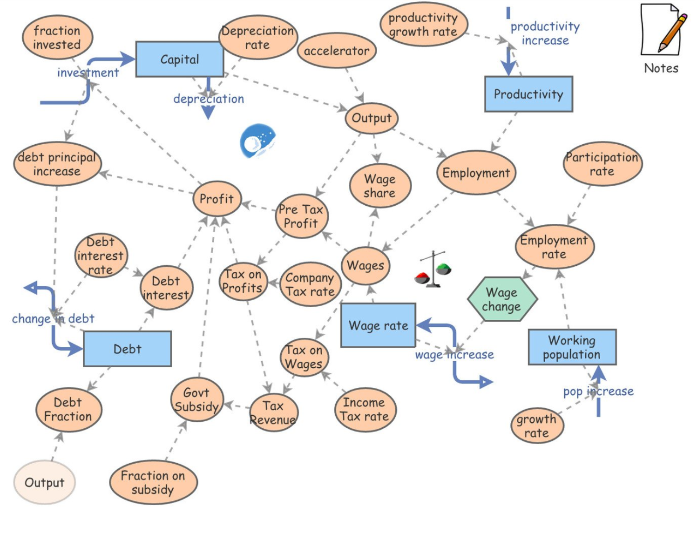
\includegraphics[width=.55\textwidth]{beamerthemesrc/images/insight-maker.png}
                \caption{Exemplo da GUI do InsightMaker.}
            \end{figure}
        \end{column}
    \end{columns}
\end{frame}


\section{Metodologia}
\begin{frame}{Fluxograma de uso simplificado}
    \begin{figure}
        \centering
        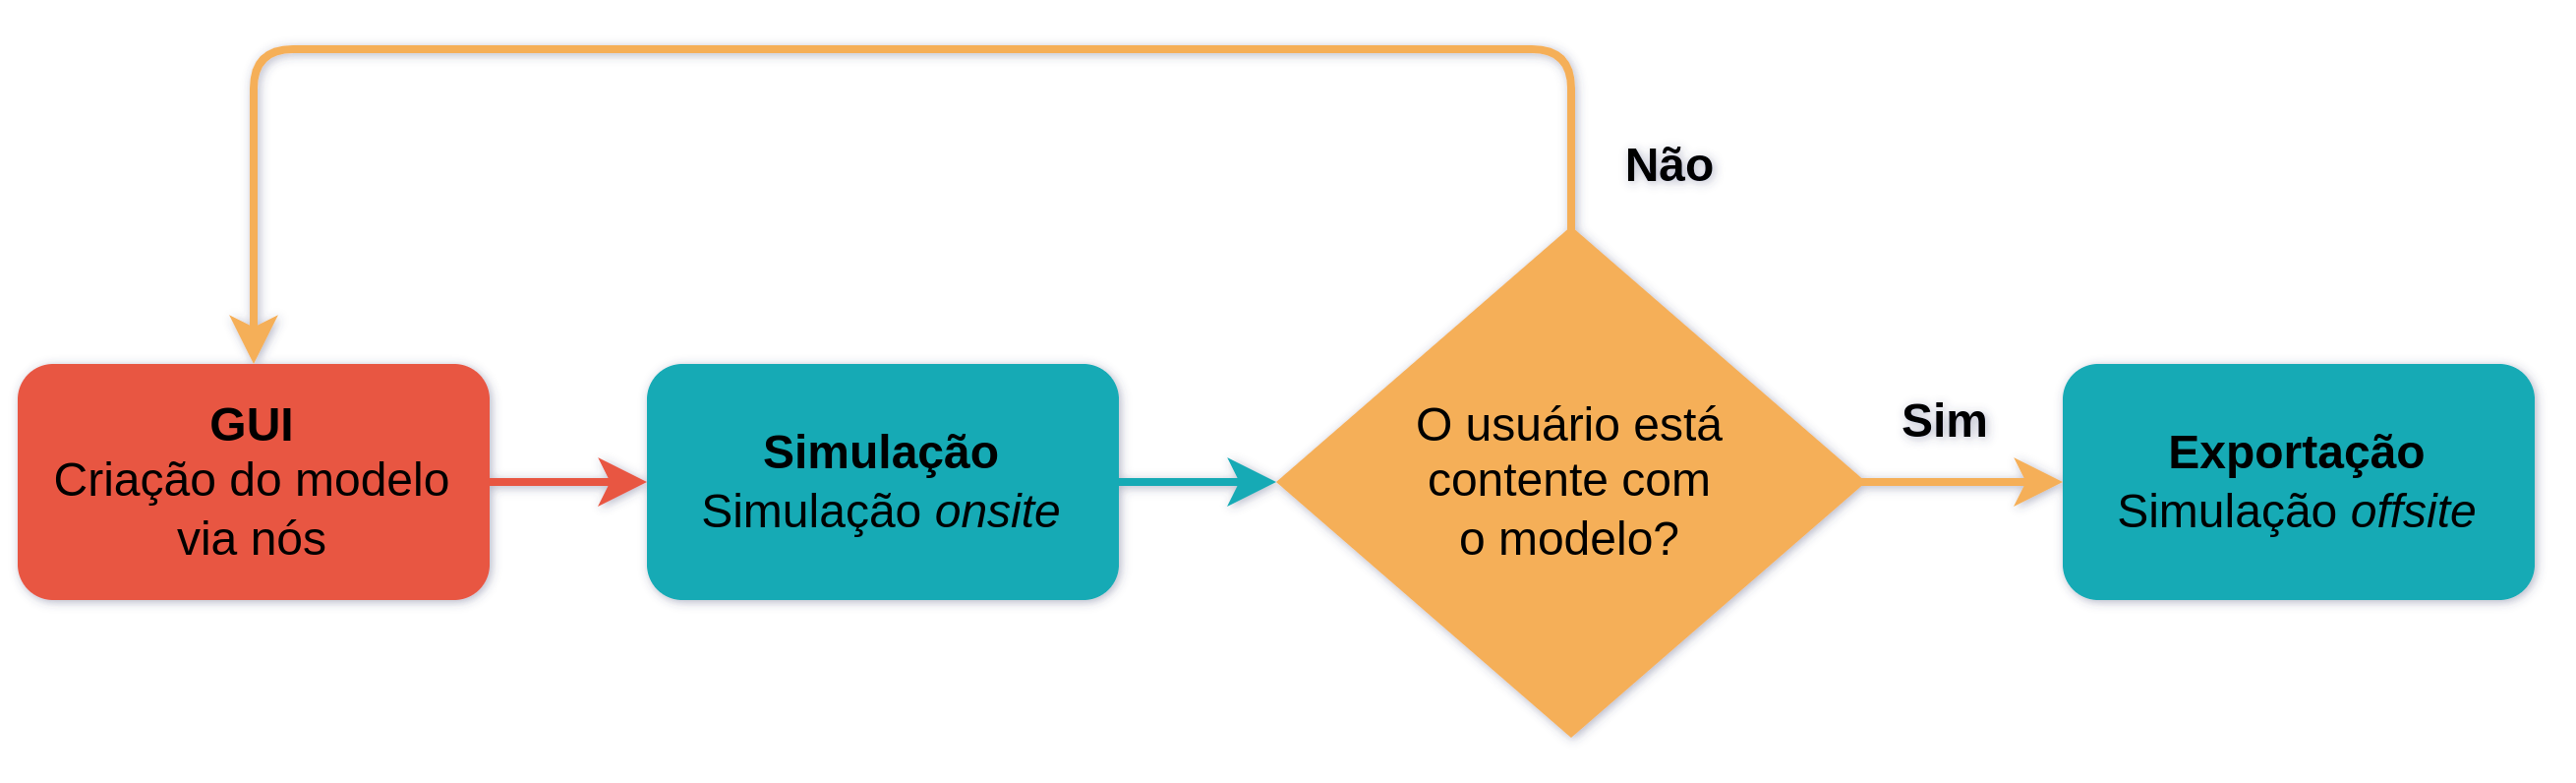
\includegraphics[width=\textwidth, height=\textheight, keepaspectratio=true]{beamerthemesrc/images/ode-designer-fluxograma.png}
        \caption{Fluxograma da experiência do usuário.}
    \end{figure}
\end{frame}

\begin{frame}{Funcionalidades do Software}
    O software deve entregar as seguintes funcionalidades:
    \begin{itemize}
        \item Criação de modelos pela interface gráfica;
        \item Simulação do modelo e exibição dos resultados na interface;
        \item Exportação de PDF/Imagens com os resultados das simulações;
        \item Exportação de código equivalente ao modelo implementado;
    \end{itemize}
\end{frame}

\subsection{Interface Gráfica}

\begin{sidepic}{beamerthemesrc/images/ode-designer-gui-exemplo}{Representação do Modelo}
    \begin{itemize}
        \item O software necessita de uma interface simples de ser usada;
            \begin{itemize}
                \item Mas também deve naturalmente relembrar uma EDO;
            \end{itemize}
        \item Após diversas iterações, chegamos numa interface baseada em programação visual;
            \begin{itemize}
                \item Estas interfaces existem desde 1963, mas tiveram uma renascença com o avanço dos computadores e a necessidade de softwares de edição de imagem/áudio/vídeo;
            \end{itemize}
    \end{itemize}
\end{sidepic}

\begin{frame}{Fluxo de passagem de informações na interface}
    \begin{figure}
        \centering
        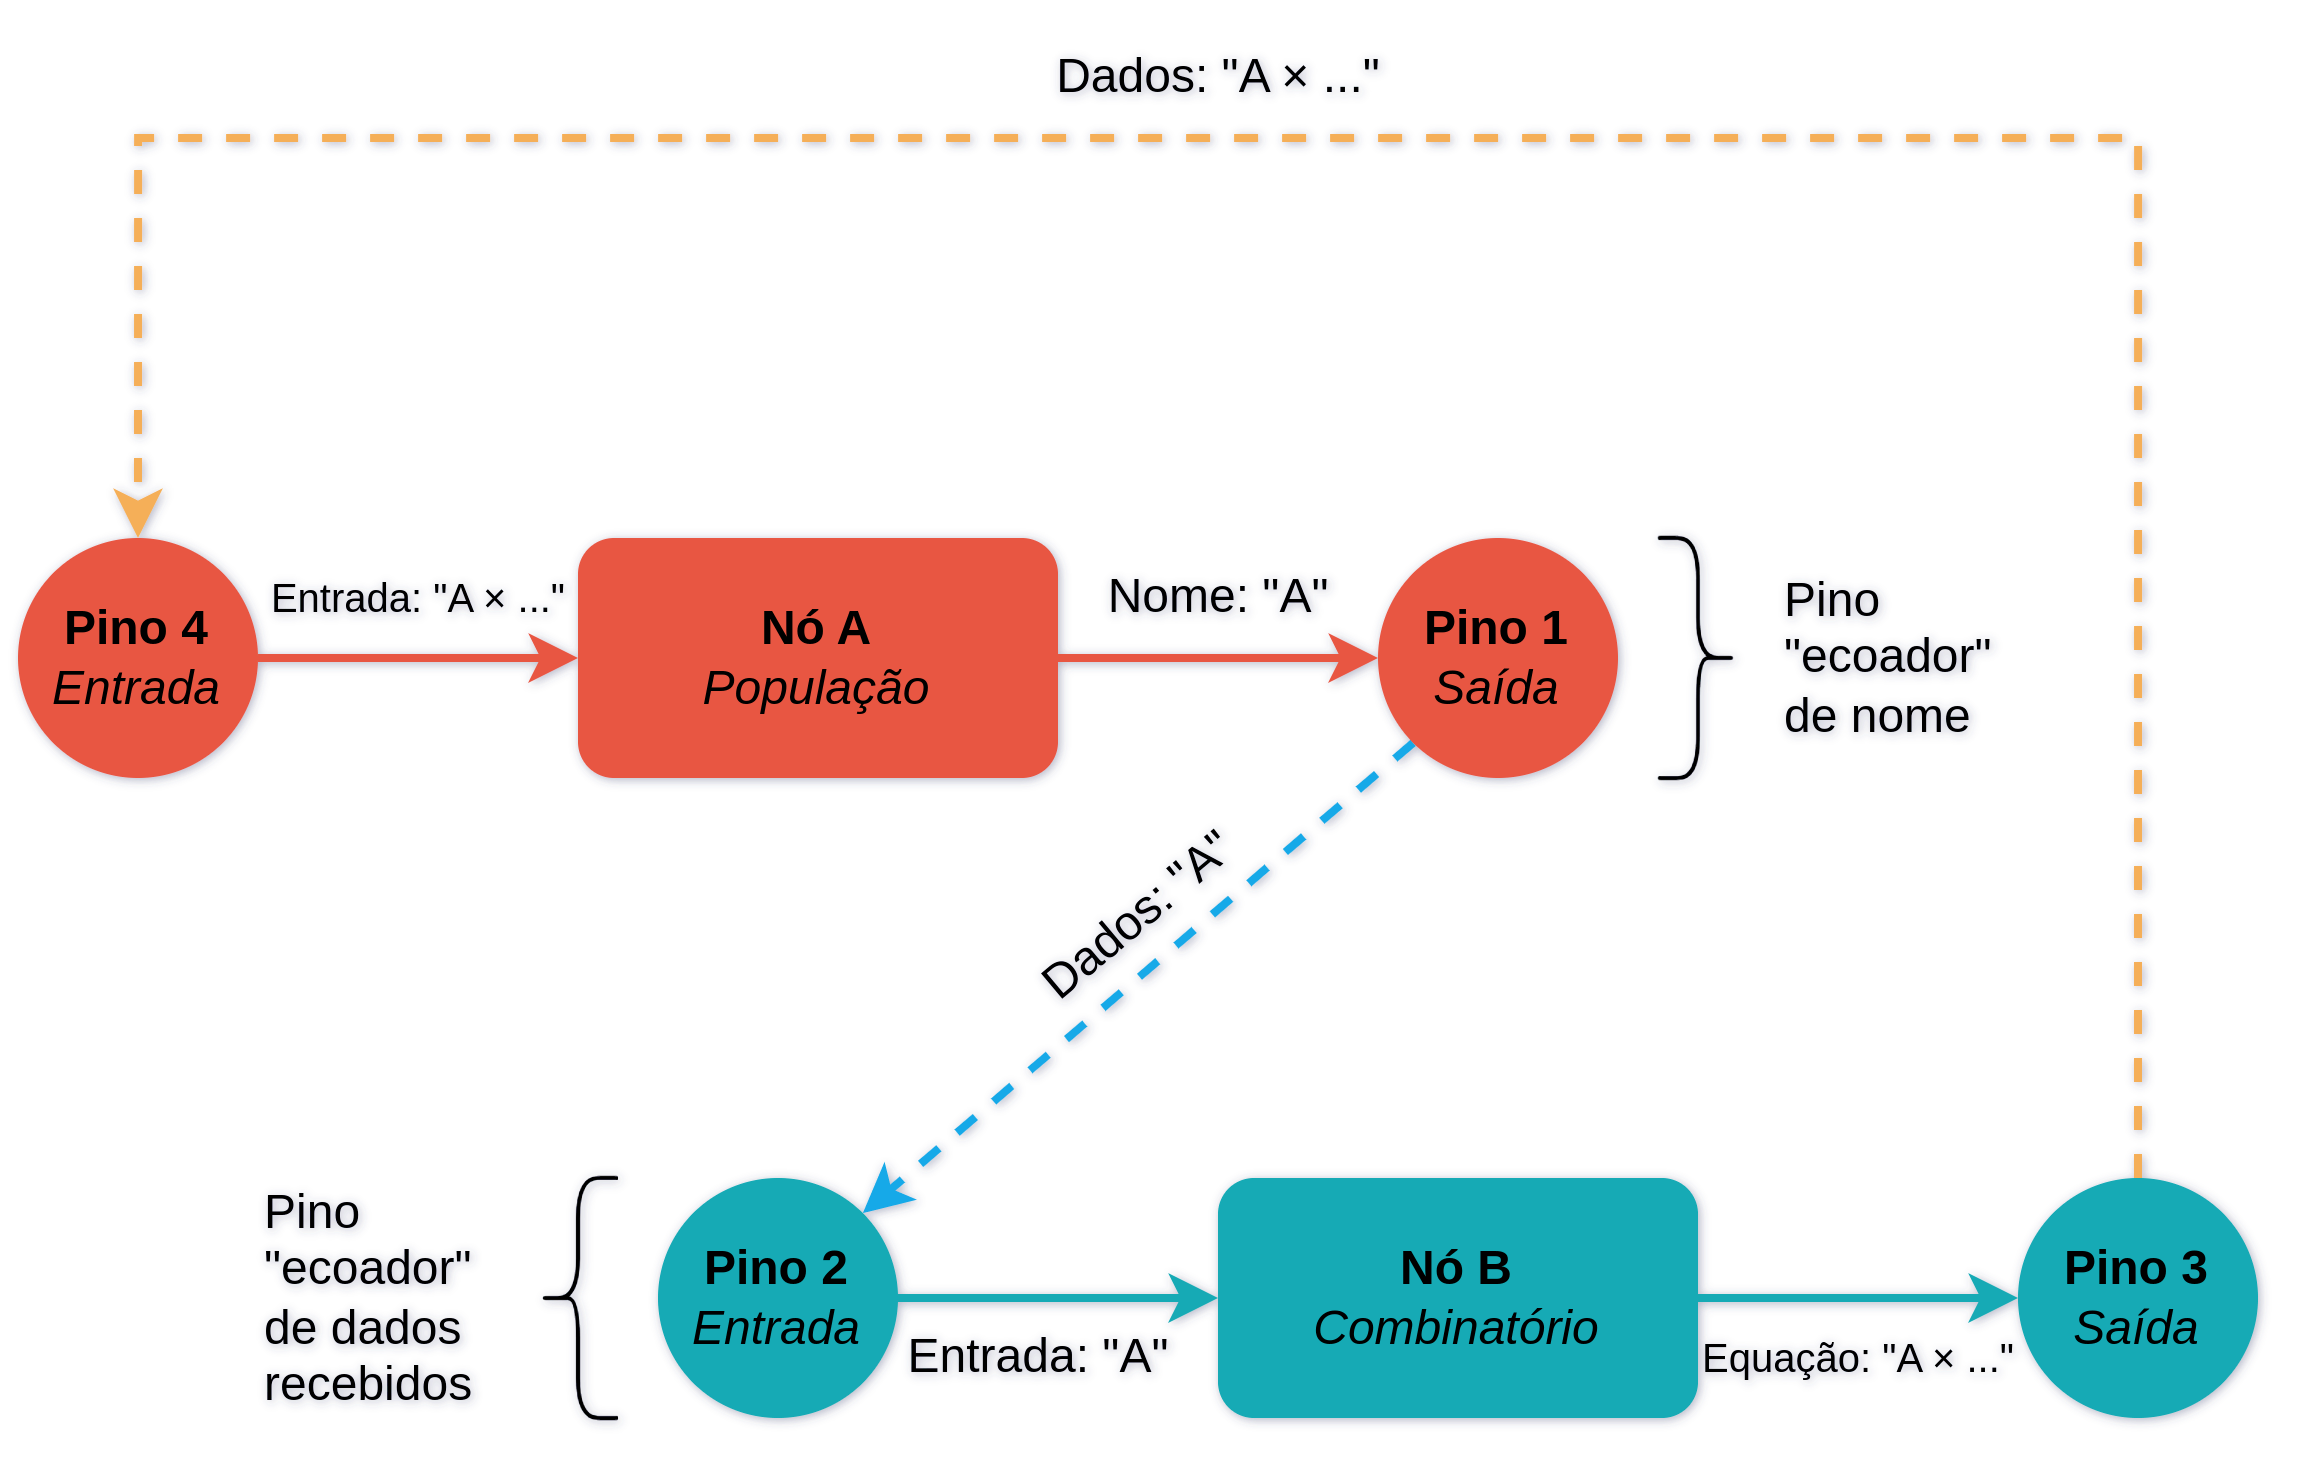
\includegraphics[width=\textwidth, height=\textheight, keepaspectratio=true]{beamerthemesrc/images/fluxo-dados-gui.png}
        \caption{Relações entre nós e pinos.}
    \end{figure}
\end{frame}

\begin{frame}{GRaIL — 1968}
    \href{https://www.youtube.com/watch?v=QQhVQ1UG6aM}{
        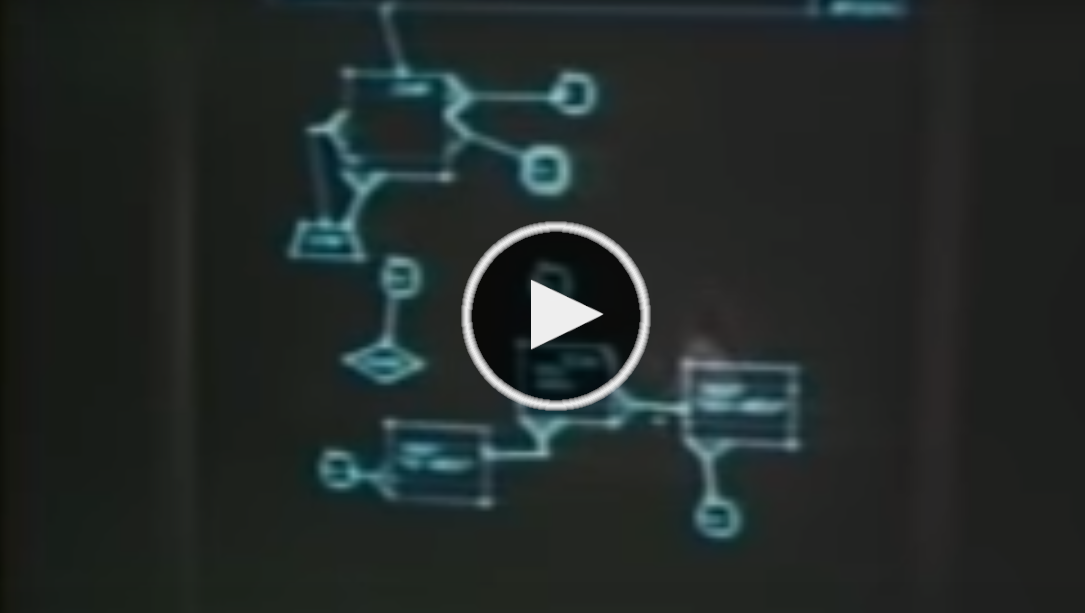
\includegraphics[width=\textwidth, height=\textheight, keepaspectratio=true]{beamerthemesrc/images/video-thumb.png}
    }
\end{frame}

\subsection{Representação Intermediária}

\begin{chapter}[beamerthemesrc/assets/background_negative]{}{Representação Intermediária}
\end{chapter}

\begin{frame}{Representação Intermediária}
    \begin{itemize}
        \item Com o objetivo de realizar tantas transformações, torna-se necessário a utilização de uma Representação Intermediária (RI);

        \item Inspirados nas arquiteturas de compiladores modernos (GCC, baseados em LLVM), separamos a estrutura em back-end e front-end;

        \item Essa abordagem garante o desacoplamento entre estrutura e produtos finais;
    \end{itemize}

    \begin{figure}
        \centering
        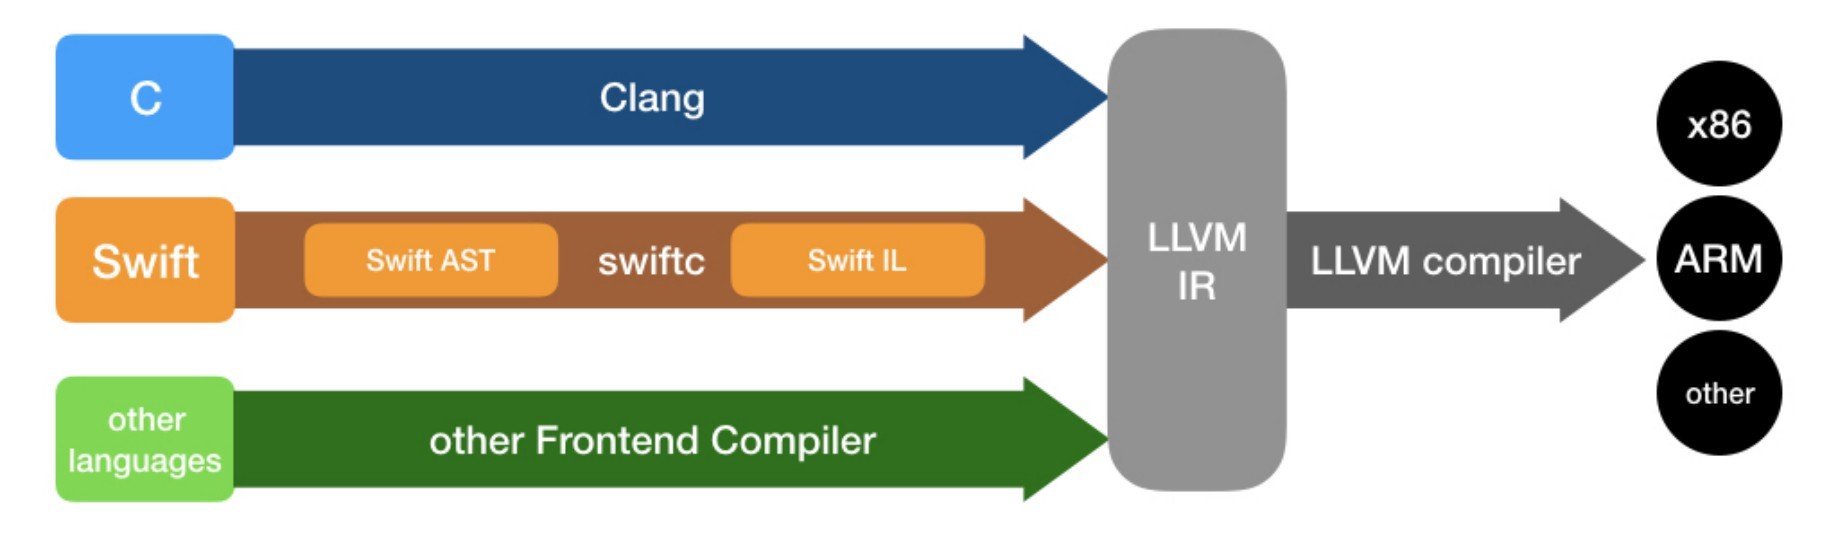
\includegraphics[height=\textheight, width=\textwidth, keepaspectratio=true]{beamerthemesrc/images/llvm-ir.png}
        \caption{Exemplo de RI: LLVM-IR.}
    \end{figure}
\end{frame}

\begin{frame}[fragile]{RI — Serde: Conversões automatizadas para JSON}
    \begin{columns}
        \begin{column}{.55\textwidth}
            \begin{block}{Rust}
                \begin{lstlisting}[language=Rust]
#[derive(Serialize, Deserialize)]
struct Person {
    name: String,
    age: u8,
    phones: Vec<String>,
    address: Address,
}
#[derive(Serialize, Deserialize)]
struct Address {
    street: String,
    city: String,
}
                \end{lstlisting}
            \end{block}
        \end{column}

        \begin{column}{.45\textwidth}
            \begin{block}{JSON}
                \begin{lstlisting}[language=json, tabsize=2]
{
  "name": "John Doe",
  "age": 43,
  "address": {
    "street": "1st St.",
    "city": "London"
  },
  "phones": [
    "+44 1234567",
    "+44 2345678"
  ]
}
                \end{lstlisting}
            \end{block}
        \end{column}
    \end{columns}
\end{frame}

\begin{frame}[fragile]{RI — \textit{Templates}}

    \begin{itemize}
        \item \texttt{Structs} \textit{serializáveis} podem ser usadas diretamente em \textit{templates};
        \item Suponha a variável \texttt{people: Vec<Person>}:
    \end{itemize}

    \begin{block}{minijinja}
        \begin{lstlisting}[language=jinja2]

    {{ person.name }}, {{ person.age }} anos.
    Contato: 
      {{ phone_nb }}
      , 
    

        \end{lstlisting}
    \end{block}
\end{frame}

\begin{frame}{Fluxo de conversões}
    \begin{figure}
        \centering
        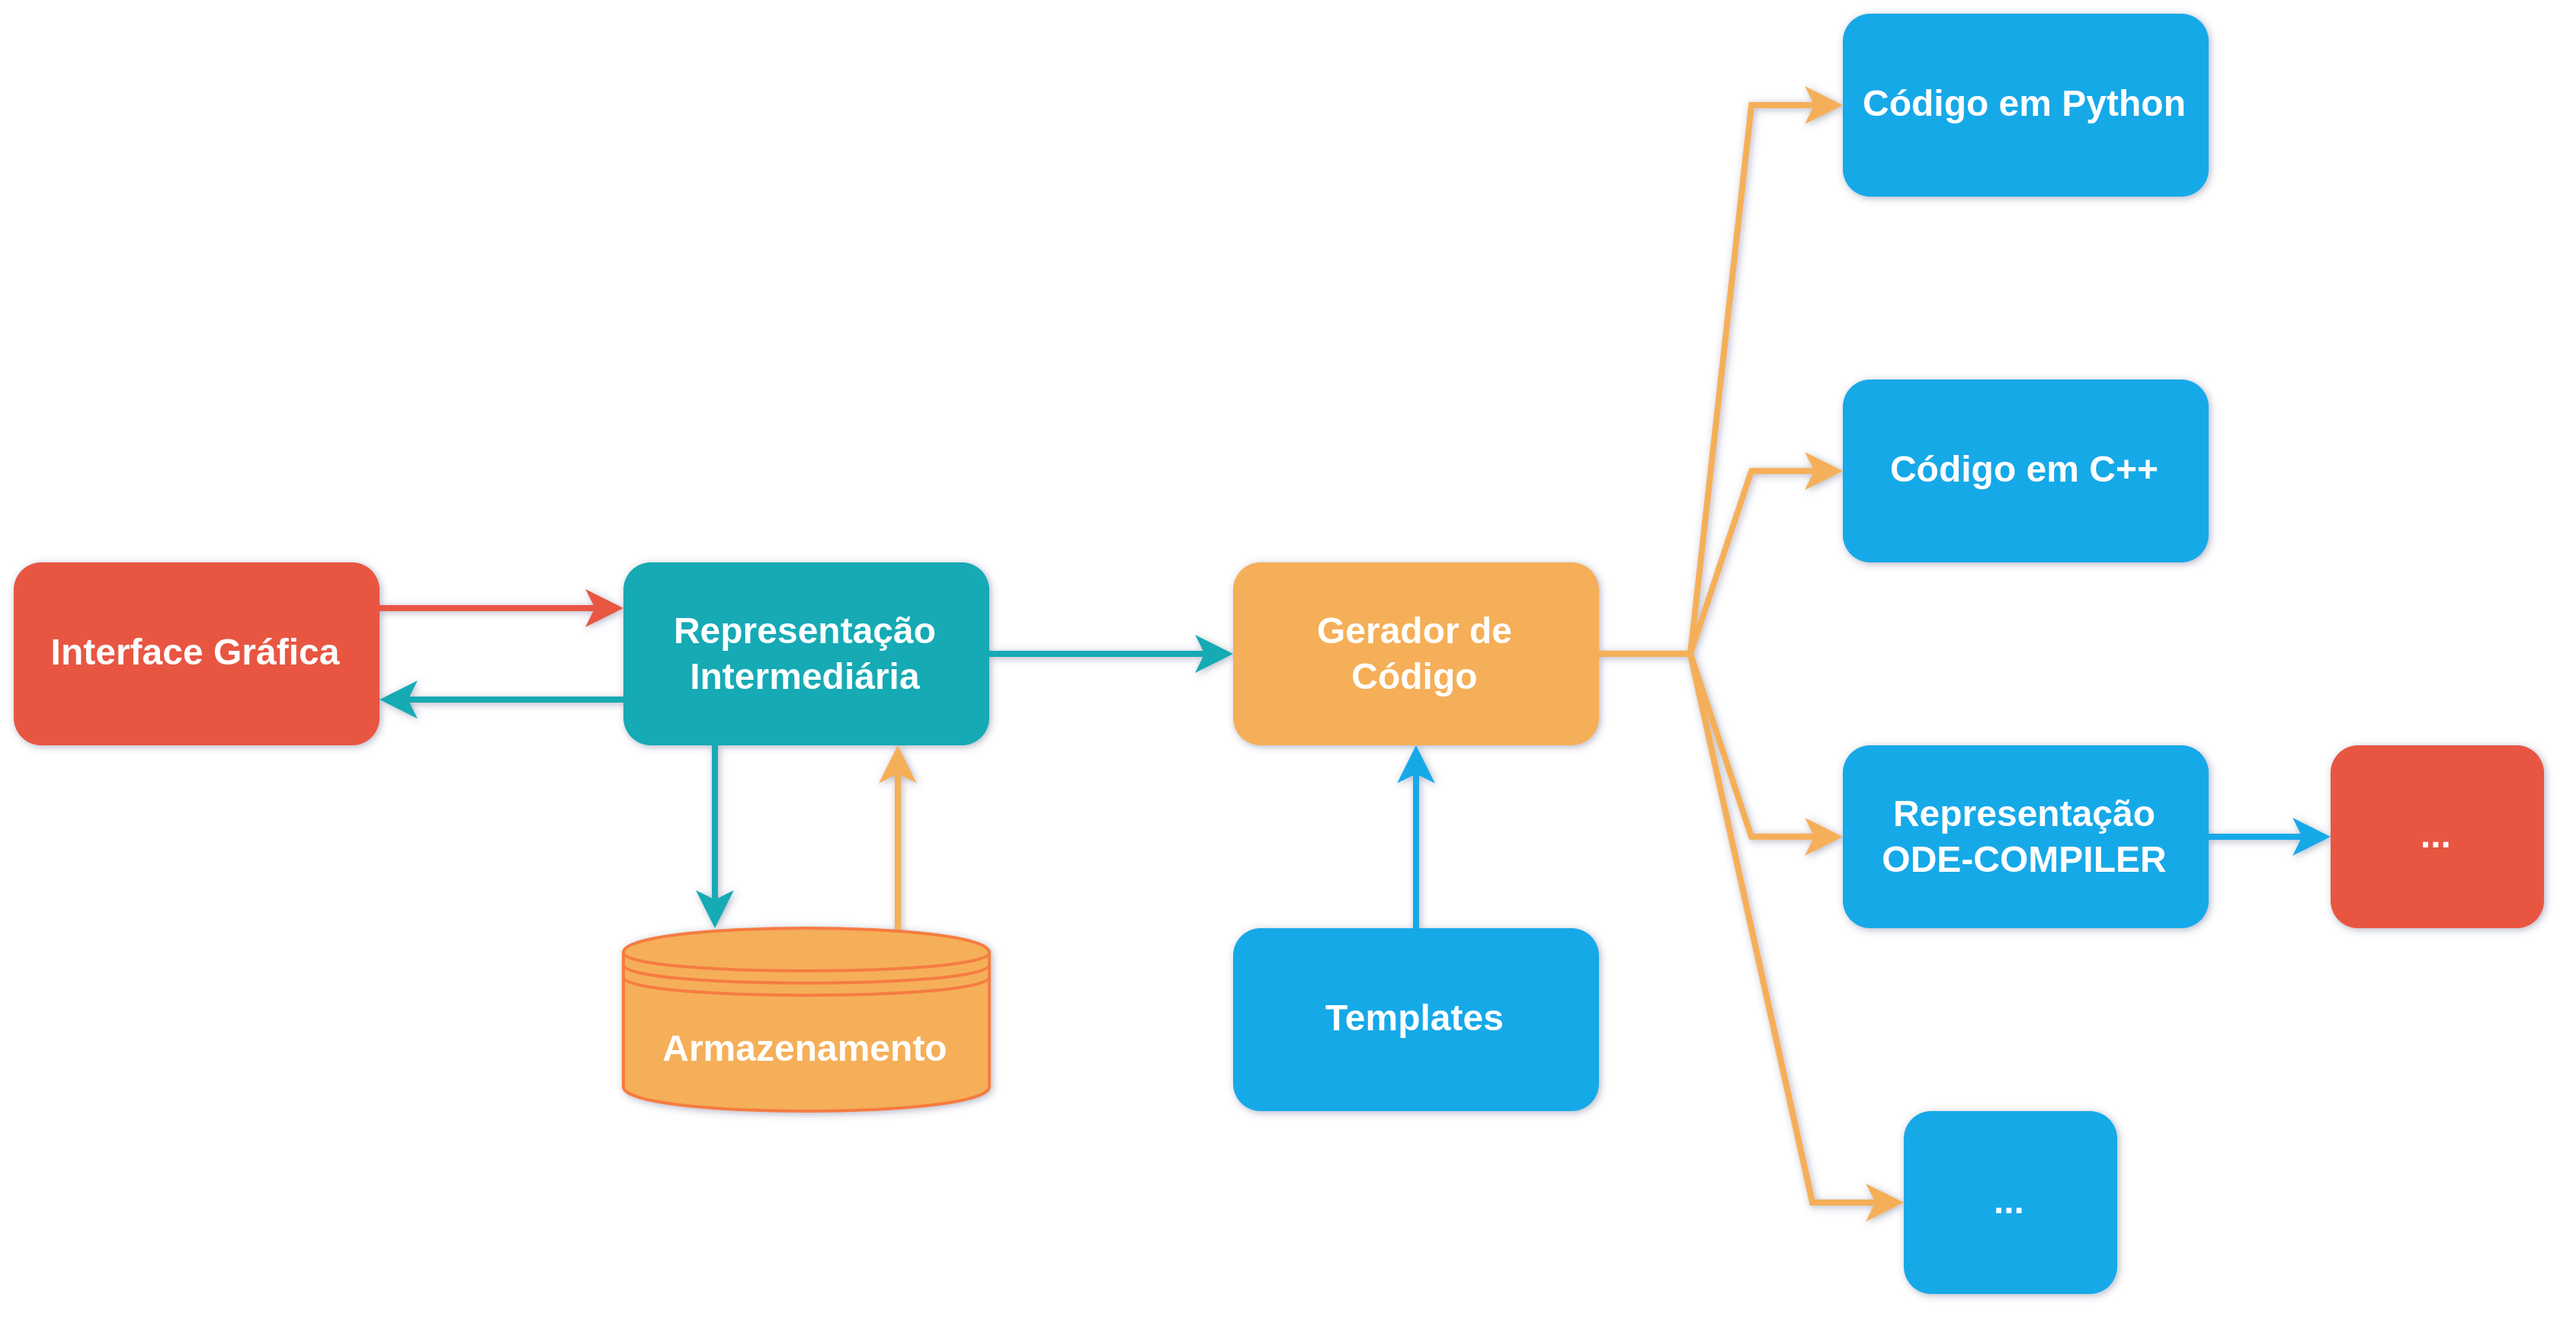
\includegraphics[width=\textwidth, height=\textheight, keepaspectratio=true]{beamerthemesrc/images/fluxo-conversoes.png}
        \caption{Fluxograma das transformações realizadas pelo software.}
    \end{figure}
\end{frame}


\section{Tecnologias Utilizadas}
\begin{frame}{Bibliotecas e Frameworks — Links}
    \begin{itemize}
        \item \hrefcol{https://github.com/Syndelis/ode-designer}{Programa Principal} / \textbf{GUI};
            \begin{itemize}
                \item C++;
                \item \hrefcol{https://www.opengl.org/}{OpenGL};
                \item \hrefcol{https://www.glfw.org/}{GLFW};
                \item \hrefcol{https://github.com/ocornut/imgui}{ImGui};
                \item \hrefcol{https://github.com/Nelarius/imnodes}{ImNodes};
                \item \hrefcol{https://github.com/epezent/implot}{ImPlot};
                \item \hrefcol{https://sciplot.github.io/}{SciPlot};
            \end{itemize}

        \item \hrefcol{https://github.com/Syndelis/odeir}{Programa Transformador} / \textbf{RI};
            \begin{itemize}
                \item Rust;
                \item \hrefcol{https://serde.rs/}{Serde};
                \item \hrefcol{https://github.com/mitsuhiko/minijinja}{minijinja};
                \item \hrefcol{https://github.com/eqrion/cbindgen}{Cbindgen};
                \item \hrefcol{https://github.com/marketplace/actions/cbindgen-action}{Cbindgen Action};
                \item \hrefcol{https://github.com/features/actions}{GitHub Actions};
                \item \hrefcol{https://github.com/catchorg/catch2}{Catch2};
            \end{itemize}
    \end{itemize}
\end{frame}


\section{Proximos Passos}
\begin{frame}{Presente}
    \begin{itemize}
        \item Iterações de design para layout da interface gráfica;
        \item Prototipagem da interface gráfica;
        \item Implementação das fundações extensíveis da interface;
        \item Implementação da Representação Intermediária e salvamento/carregamento de arquivos do computador;
        \item Testes de integração entre GUI e RI;
    \end{itemize}
\end{frame}

\begin{frame}{Futuro}
    \begin{enumerate}
        \item \label{cro::geracao-codigo-python-I} Geração de código em Python;
        \item \label{cro::exportacao-pdf-II} Exportação dos resultados das simulações em PDF;
        \item \label{cro::testes-III} Testes do software através da construção de diversos modelos da literatura;
        \item \label{cro::simulacao-onsite-IV} Integração com odecompiler e implementação da simulação interativa com exibição de gráficos em tempo real;
        \item \label{cro::gillespie-V} Definição do template e implementação da geração de código para o algoritmo de Gillespie; 
        \item \label{cro::artigo-VI} Escrita de artigo para publicação em revista; 
        \item \label{cro::escrita-dissertacao-VII} Escrita do texto final da dissertação de Mestrado.
    \end{enumerate}
\end{frame}

\begin{frame}[fragile]{Cronograma}
    \begin{table}
        \centering
            \begin{tabular}{|c|c|c|c|c|c|c|c|c|c|c|c|}
            \hline
            &\multicolumn{5}{c|}{2023}&\multicolumn{1}{c|}{2024}\\
            \hline
                &\nicefrac{Mar}{Abr}&\nicefrac{Mai}{Jun}&\nicefrac{Jul}{Ago}&\nicefrac{Set}{Out}&\nicefrac{Nov}{Dez}&\nicefrac{Jan}{Fev}\\
            \hline
            \ref{cro::geracao-codigo-python-I}&\cellcolor{midgray}&\cellcolor{midgray}&&&&\\
                \hline
                \ref{cro::exportacao-pdf-II}&&\cellcolor{midgray}&&&&\\
                \hline
                \ref{cro::testes-III}&\cellcolor{midgray}&\cellcolor{midgray}&\cellcolor{midgray}&\cellcolor{midgray}&\cellcolor{midgray}&\\
                \hline
                \ref{cro::simulacao-onsite-IV}&&&\cellcolor{midgray}&\cellcolor{midgray}&\cellcolor{midgray}&\\
                \hline
                \ref{cro::gillespie-V}&&&&\cellcolor{midgray}&\cellcolor{midgray}&\\
                \hline
                \ref{cro::artigo-VI}&&&\cellcolor{midgray}&\cellcolor{midgray}&\cellcolor{midgray}&\cellcolor{midgray}\\
                \hline
                \ref{cro::escrita-dissertacao-VII}&&&&&\cellcolor{midgray}&\cellcolor{midgray}\\
                \hline
            \end{tabular}
    \end{table}
\end{frame}

\backmatter
\end{document}
